\chapter{Les phénomènes périodiques}
La révolution de la Terre, un enfant sur une balançoire, une roue qui tourne, les battements du c\oe{}ur, \ldots de nombreux phénomènes du quotidien se répètent toujours de la même manière, ils présentent un \motcle{caractère périodique}.

Parmi les phénomènes périodiques, certains consistent en un va-et-vient autour d'une position d'équilibre : la balançoire, une latte qui vibre au bord d'un bureau, un ressort avec une masse à son extrémité, ce sont des phénomènes d'\motcle{oscillation}.
\begin{figure}[h!]
    \begin{minipage}{.5\textwidth}
        \centering
        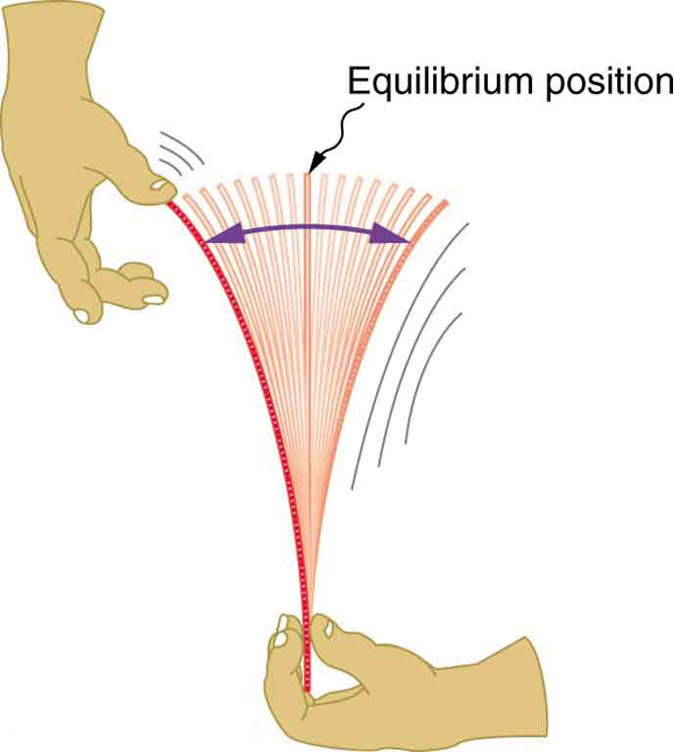
\includegraphics[width=.8 \linewidth]{latte_vibre.png}
        %\includesvg[inkscapelatex=false, width=.5 \linewidth]{tir_oblique.svg}
        \caption{Une tige rigide vibrant par rapport à sa position de repos est un oscillateur.}
        \label{lame_vibre}
    \end{minipage}
    \begin{minipage}{.5\textwidth}
        \centering
        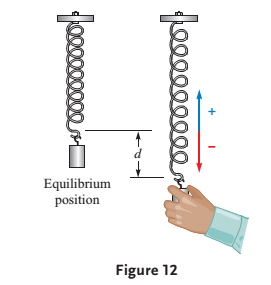
\includegraphics[width=.8 \linewidth]{ressort_oscille.png}
        \caption{Une masse attachée à un ressort est un exemple très classique d'oscillateur.}
        \label{lame_vibre_2}
    \end{minipage}
\end{figure}

\newpage

\section{Caractéristiques des oscillateurs}
Lorsqu'on cherche à étudier un phénomène, il est indispensable de prendre conscience des paramètres qui le caractérise afin de pouvoir mesurer ceux-ci.
Après avoir observé le pendule qui oscille, précise quels sont les paramètres caractéristiques des phénomènes d'oscillation.
\begin{itemize}[label=\textbullet]
    \item Élongation : \dotfill
          \pointilles{2}
    \item Amplitude : \dotfill
          \pointilles{2}
    \item Fréquence : \dotfill
          \pointilles{2}
    \item Période : \dotfill
          \pointilles{2}
\end{itemize}

\newpage

\section{La bouteille d'encre}
Une bouteille remplie d'encre ou de peinture oscille au-dessus d'une feuille de papier. Une ouverture de faible diamètre est pratiquée sous la bouteille de manière que le liquide qu'elle contient tombe goutte à goutte sur la feuille. Si on laisse la bouteille osciller, une ligne apparaît sur la feuille, chaque goutte qui tombe sur le papier indique l'élongation du pendule.
Si la feuille est déplacée sous la bouteille à vitesse constante alors le liquide qui s'écoule ne dessine plus une droite, la figure qui apparaît sur le papier est une sinusoïde.

\begin{figure}[h!]
    \begin{minipage}{.5\textwidth}
        \centering
        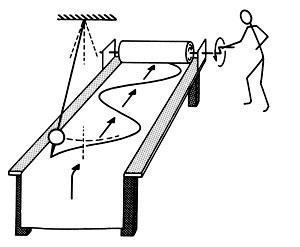
\includegraphics[width=.8 \linewidth]{bouteille_encre1.png}
        \caption{L'élongation d'un pendule en fonction du temps est une sinusoïde.}
        \label{bouteille_encre1}
    \end{minipage}
    \begin{minipage}{.5\textwidth}
        \centering
        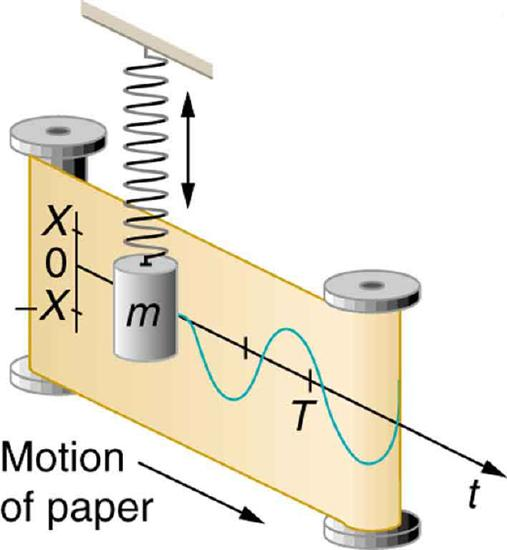
\includegraphics[width=.8 \linewidth]{bouteille_encre2.png}
        \caption{L'élongation du système masse-ressort en fonction du temps est aussi un sinusoïde.}
        \label{bouteille_encre2}
    \end{minipage}
\end{figure}

\begin{encadre}
    Un \motcle{mouvement harmonique} est un mouvement d'oscillation dont la représentation de l'élongation au cours du temps est une fonction sinusoïdale.
\end{encadre}

\newpage

\section{Exemples de mouvements simples harmoniques (MSH - SHM)}
\begin{figure}[h!]
    \centering
    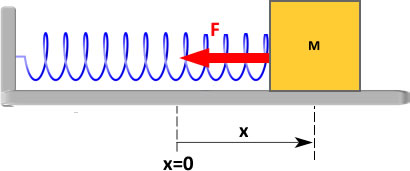
\includegraphics[width=.8 \linewidth]{bloc_ressort.png}
    \caption{Système bloc-ressort horizontal.}
    \label{bloc_ressort}
\end{figure}

\begin{figure}[h!]
    \begin{minipage}{.5\textwidth}
        \centering
        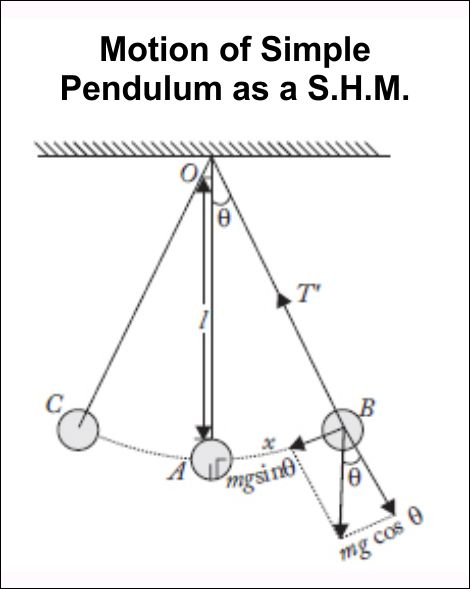
\includegraphics[width=.8 \linewidth]{pendule.png}
        \caption{Un pendule simple.}
        \label{pendule}
    \end{minipage}
    \begin{minipage}{.5\textwidth}
        \centering
        \includegraphics[width=.8 \linewidth]{bloc_ressort_2.png}
        \caption{Système bloc-ressort vertical.}
        \label{bouteille_encre3}
    \end{minipage}
\end{figure}

\newpage

\section{Le point sur le disque}
Un observateur s'intéresse à la position verticale d'un point placé sur un disque en rotation. Si le disque tourne avec une vitesse angulaire de \(\omega [rad \cdot s^{-1}]\) alors la position verticale est donnée par
\begin{equation}
    \tcboxmath[colback=LightBlue,colframe=blue]
    {x(t)=A \cdot sin(\omega t)}
\end{equation}.

\begin{figure}[h!]
    \centering
    %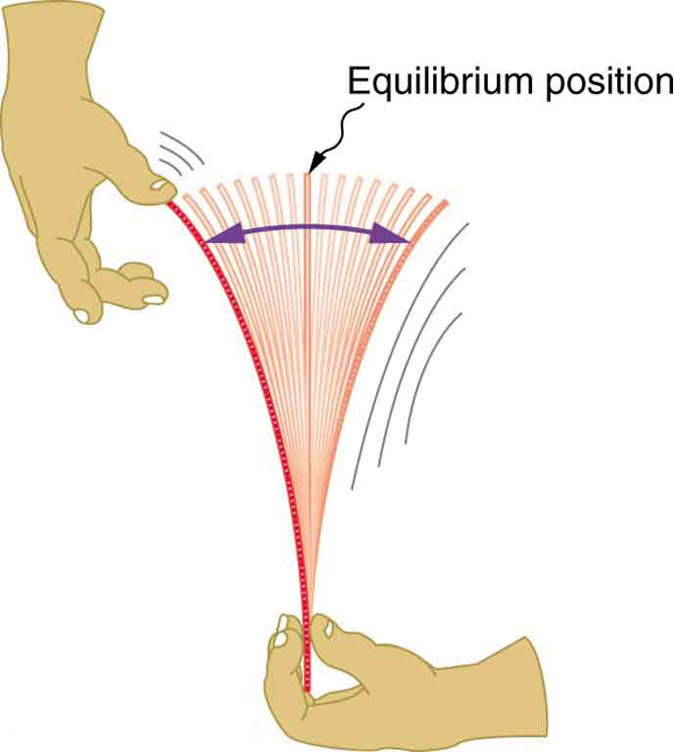
\includegraphics[width=.8 \linewidth]{latte_vibre.png}
    \includesvg[inkscapelatex=false, width=.5 \linewidth]{disque_tournant.svg}
    %\caption{}
    %\label{}
\end{figure}


Le mouvement d'un point sur un disque n'est pas l'exemple le plus évident de mouvement harmonique, mais il est facile à aborder sur le plan mathématique. Un observateur regardant le disque de côté verra le point monter et descendre comme une masse sur un ressort ou comme un pendule.
Dans le cas des mouvements harmoniques, le facteur \(\omega\) est appelé \motcle{pulsation} ou \motcle{fréquence angulaire}, il détermine le nombre de passages par la position d'équilibre que le système effectue à chaque seconde.

\newpage

\subsection{Une nouvelle vision de la vitesse et de l'accélération}
Lors des premiers cours de cinématique, la vitesse moyenne a été définie comme : \(v_{moy}=\frac{\Delta x}{\Delta t}\). Comme son nom l'indique, la vitesse moyenne est une valeur moyenne mesurée sur un intervalle de temps. Si la valeur de la vitesse moyenne est suffisante dans de nombreuses situations, il est souvent utile de connaître la valeur de la vitesse à un instant précis, c'est-à-dire la \motcle{vitesse instantanée}.
La vitesse instantanée est la valeur de la vitesse moyenne prise sur un intervalle de temps infiniment cours :\(v_{inst}= lim_{\Delta t \rightarrow 0} \frac{\Delta x}{\Delta t}\). Cela correspond à la dérivée de la position.

\begin{encadre}
    En physique, la vitesse est toujours définie comme étant la dérivée de la position par rapport au temps.
\end{encadre}

De même, l'accélération moyenne est donnée par : \(a_{moy}=\frac{\Delta v}{\Delta t}\) et l'accélération instantanée se trouve en faisant : \(a_{inst}= lim_{\Delta t \rightarrow 0} \frac{\Delta v}{\Delta t}\).

\begin{encadre}
    En physique, l'accélération est toujours définie comme étant la dérivée de la vitesse par rapport au temps.
\end{encadre}

Avec le raisonnement inverse, on comprend que la vitesse peut être trouvée en faisant l'intégrale de l'accélération et la position en faisant l'intégrale de la vitesse.

\subsection{Vérification}
L'équation horaire de la position dans le MRUA était donnée par : \(x(t)=x_0 + v_0 \cdot \Delta t + \frac{a}{2} \cdot \Delta t^2\).
La dérivée de cette fonction par rapport au temps donne : \(x'(t)=v(t)=v_0 + a \cdot \Delta t\)
Et la dérivée de celle-ci donne : \(x''(t)=v'(t)=a(t)=a\)

\begin{itemize}[label=$\rightarrow$]
    \item Détermine l'équation de la vitesse et celle de l'accélération pour le mouvement simple harmonique.
          \pointilles{5}
\end{itemize}

\newpage

\section{Le déphasage}
Que se passe-t-il si l'objet étudié n'est pas à la position \enquote{0} à l'instant \enquote{0} ?

Dans ce cas, l'écart par rapport à la position d'équilibre, appelé \motcle{constante de phase} ou \motcle{déphasage} se note \(\phi\) et l'équation de la position s'écrit :
\begin{equation}
    \tcboxmath[colback=LightBlue,colframe=blue]
    {x(t)=A \cdot sin(\omega t + \phi)}
\end{equation}

\begin{figure}[h!]
    \centering
    %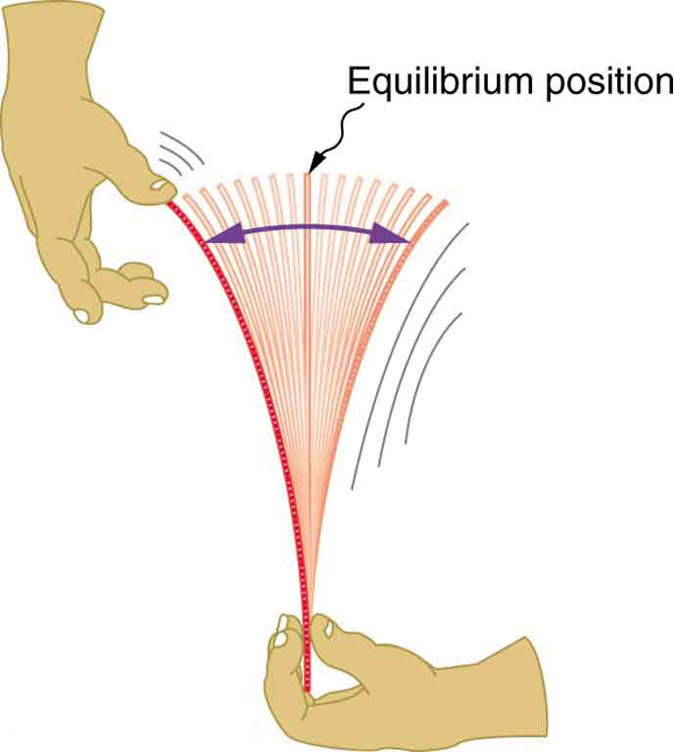
\includegraphics[width=.8 \linewidth]{latte_vibre.png}
    \includesvg[inkscapelatex=false, width=.5 \linewidth]{disque_tournant_phase.svg}
    %\caption{}
    %\label{}
\end{figure}

\newpage

\section{Exercices}
\begin{exercise}
    La position d'une particule est donnée par \(x(t)=0,03 \cdot sin(20 \pi t + \frac{\pi}{4})\)
    \begin{enumerate}[a)]
        \item Dans cette équation, identifie l'amplitude, la pulsation, le déphasage.
        \item Détermine à quel moment la position, la vitesse et l'accélération atteignent une valeur maximale positive.
    \end{enumerate}
\end{exercise}

\begin{exercise}
    Un oscillateur harmonique a pour équation de l'élongation : \(y(t)=6sin(3 \pi \cdot t + \frac{\pi}{3})\) où t est donné en secondes et y en centimètres.
    \begin{enumerate}[a)]
        \item Calcule la période du mouvement harmonique, sa fréquence et sa constante de phase.
        \item Écris l'équation de la vitesse et calcule la vitesse en \(t=3[s]\).
        \item Écris l'équation de l'accélération et calcule l'accélération en \(t=3[s]\).
    \end{enumerate}
\end{exercise}

\begin{exercise}
    Le piston d'un moteur à explosion effectue 3000 oscillations par minute.
    \begin{enumerate}[a)]
        \item Calcule sa fréquence et sa période.
        \item Si le mouvement est harmonique et que l'amplitude vaut \(5cm\), calcule la vitesse maximale du piston.
        \item Calcule son accélération maximale.
        \item Si la masse du piston est de \(100g\), calcule la force maximale s'exerçant sur lui.
    \end{enumerate}
\end{exercise}

Exercices supplémentaires :\\
\qrcode{https://www.vf-bxl-moodle.be/mod/quiz/view.php?id=1370}


\newpage

\section{Caractéristiques du MSH}
Nous allons mettre en évidence les conditions dans lesquelles un mouvement simple harmonique apparaît.
L'équation horaire de l'accélération montrait que \(a(t)=- \omega ^2 \cdot  x(t)\). Si on souhaite connaître la façon dont la force qui crée le SHM varie, on obtient : \(F(t)=- m \cdot \omega ^2 \cdot x(t)\). Les paramètres \(m\) et \(\omega\) sont constants, donc le produit \(m \cdot \omega\) aussi une constante. Il est donc permis d'écrire : \(F(t)=- k \cdot x(t)\).

Cette dernière équation montre que dans un MSH :
\begin{enumerate}[(a)]
    \item la force qui crée le mouvement est proportionnelle à l'élongation ;
    \item cette force est opposée à l'élongation, c'est une \motcle{force de rappel}.
\end{enumerate}


Toute situation dans laquelle une telle force est observée va engendrer un MSH. De la même manière, une situation dans laquelle il existe une force constante centripète crée un MCU ou une situation dans laquelle il existe une force constante dans le sens du déplacement crée un MRUA.


\begin{figure}[h!]
    \centering
    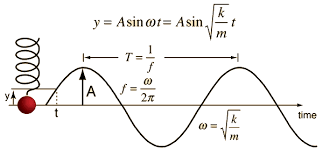
\includegraphics[width=.5 \linewidth]{shm.png}
    %\includesvg[inkscapelatex=false, width=.5 \linewidth]{tir_oblique.svg}
    \caption{Un mouvement simple harmonique}
    \label{shm}
\end{figure}
